\heading{177neV parxkaraNa}

\subheading{gajAnayana leKaKxvu}

\begin{description}
\item[$(1)$ u.] kelavu AnegaLu mUru mAgaRgaLalilx hoVgutAtx idudx, A
  meVle $1$kekx mUraraSATxgi $5$ keregaLalilx niVru kuDidavu. AnaMtara
  $1$kekx $5$raSaTxgi $7$ kADugaLige meVyuvadakekx hoVdavu. taruvAya
  $1$kekx $7$raSaTxgi $9$ beTaTxgaLige hokakxvu. alilx $1$kekx
  $9$raSATxgi $11$ kabibxna gadedxgaLanunx parxveVshisidavu. alilxMda
  $1$kekx $11$raSATxgi $13$ deVshagaLige horaTu hoVdavu. Adare modalu
  idadx AnegaLeSuTx? matutx leKaKxda parxkArakekx eSeTxSuTx AnegaLu
  yAvAyxva kaqtayxgaLanunx naDisidavu. aMdare, sUtarx.

\item[kaM||] BAgagaLelalxva niriya| lAkxguvadAdi
  gajaMgaLavanaMmatAtx|| AgirutihamaMshagaLoLu|
  beVgadiguNisutatxladara BAgadoLehxriseY||

\item[vi||] BAgagaLa saMKayxgaLanunx parasapxravAgi guNisidare, baruva
  labadxveV Adiyalilxdadx gajagaLAvuvu. taruvAya adanunx AyAya
  aMshagaLiMda guNisi, adaradara CeVdagiMda BAgisutAtx hoVdare, AyAyA
  kaqtayxgaLanunx mADidaMthA gajagaLAguvavu.

\item[riVti] $\dfrac{1}{3}$, $\dfrac{3}{5}, \dfrac{5}{7}, \dfrac{7}{9},
  \dfrac{9}{11}, \dfrac{11}{13}$ ivugaLa CeVdagaLelAlx parasapxravAgi
  guNisalu, 

  $3 \times 5 \times 7 \times 9 \times 11 \times 13= 135135$
  iveV Adiyalilxdadx gajagaLU.
 \begin{figure}[H]
  \centerline{ 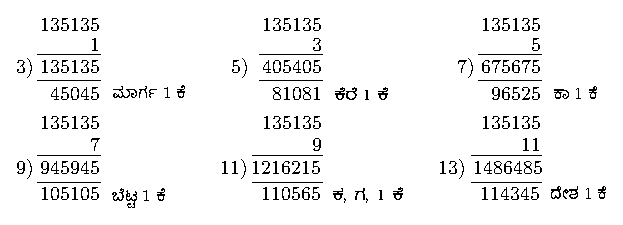
\includegraphics{images/177.eps}}
 \end{figure}

\end{description}
